\documentclass[a4paper]{article}
\usepackage[a4paper, total={6in, 8in}]{geometry}
\usepackage{float}
\usepackage{amsmath, amssymb, amsthm, amsfonts, bm, commath}
\usepackage{physics}
\usepackage{tikz}
\usetikzlibrary{positioning, calc, math, shapes, fit, arrows, decorations.pathreplacing, decorations.text, intersections}
\usepackage{pgfplots}
\usepgfplotslibrary{fillbetween}

\begin{document}
This is an example test, showing a reproduction of a figure from a textbook. See Figure \ref{fig:frank-condon} for more info.

\begin{figure}[H]
  \centering
  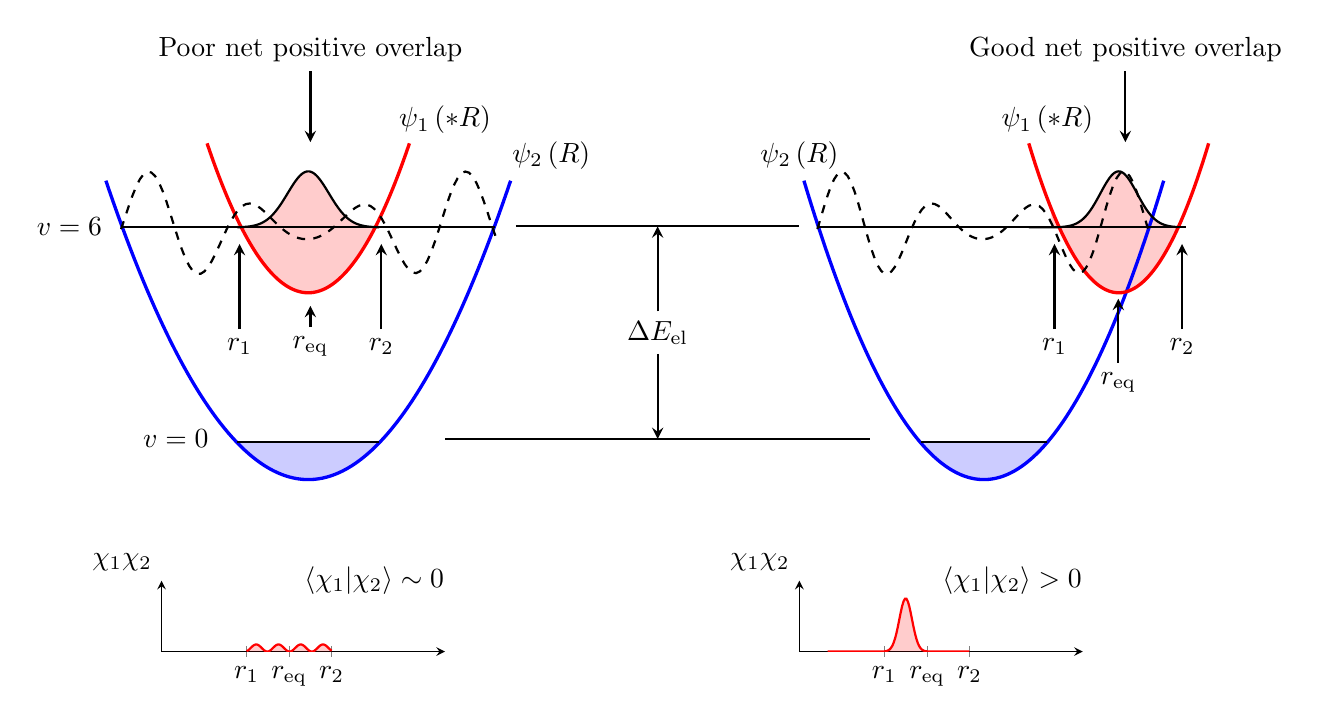
\begin{tikzpicture}[scale=0.9]
  \tikzset{line/.style={thick, black}}
  \tikzset{arrow/.style={->, >=stealth, thick, black}}
  \tikzset{function/.style={very thick, samples=100}}

  % Center part
  \draw[line] (-3,0) -- (3,0);
  \draw[line] (-2,3) -- (2,3);
  \node (E1) at (0,1.5) {$\Delta E_{\text{el}}$};
  \draw[arrow] (E1.south) -- (0,0);
  \draw[arrow] (E1.north) -- (0,3);

  % Left functions
  \begin{axis}[at={(-8.3cm,-1cm)},
	 domain=-5:5,
	 ticks=none,
	 axis line style={draw=none}]
	 \addplot[name path=par1, function, blue, domain=-4:4] {x^2};
	 \addplot[name path=par2, function, red, domain=-2:2] {2*x^2+10};
	 \addplot[name path=line1, function, thick, domain=-1.4:1.4] {2};
	 \addplot[name path=line2, function, thick, domain=-3.7:3.7] {13.5};
	 \addplot[name path=exp, function, thick, domain=-1.4:1.4] {3*exp(-3*x^2)+13.5};
	 \addplot[name path=sine, function, thick, dashed, domain=-3.7:3.7] {sin(deg(3*x-1.5))*3*(exp(-(x+3)^2/4)+exp(-(x-3)^2/4))+13.5};
	 \addplot[thick, color=blue, fill=blue, fill opacity=0.2] fill between[of=par1 and line1, soft clip={domain=-1.4:1.4}];
	 \addplot[thick, color=red, fill=red, fill opacity=0.2] fill between[of=par2 and exp, soft clip={domain=-1.4:1.4}];
  \end{axis}
  \node[align=center] (poor) at (-4.9,5.5) {Poor net positive overlap};
  \draw[arrow] (poor.south) -- ++(0,-1);
  \node at (-6.8,0) {$v=0$};
  \node at (-8.3,3) {$v=6$};
  \node at (-3,4.5) {$\psi_{1}\left( *R \right)$};
  \node at (-1.5,4) {$\psi_{2}\left( R \right)$};
  \node (r1) at (-5.9,1.3) {$r_{1}$};
  \node (req) at (-4.9,1.3) {$r_{\text{eq}}$};
  \node (r2) at (-3.9,1.3) {$r_{2}$};
  \draw[arrow] (r1.north) -- ++(0,1.2);
  \draw[arrow] (req.north) -- ++(0,0.3);
  \draw[arrow] (r2.north) -- ++(0,1.2);
  

  % Right functions
  \begin{axis}[at={(1.55cm,-1cm)},
	 ticks=none,
	 axis line style={draw=none}]
	 \addplot[name path=par1, function, blue, domain=-4:4] {x^2};
	 \addplot[name path=par2, function, red, domain=1:5] {2*(x-3)^2+10};
	 \addplot[name path=line1, function, thick, domain=-1.4:1.4] {2};
	 \addplot[name path=line2, function, thick, domain=-3.7:4.5] {13.5};
	 \addplot[name path=exp, function, thick, domain=1:4.3] {3*exp(-3*(x-3)^2)+13.5};
	 \addplot[name path=sine, function, thick, dashed, domain=-3.7:3.7] {sin(deg(3*x-1.5))*3*(exp(-(x+3)^2/4)+exp(-(x-3)^2/4))+13.5};
	 \addplot[thick, color=blue, fill=blue, fill opacity=0.2] fill between[of=par1 and line1, soft clip={domain=-1.4:1.4}];
	 \addplot[thick, color=red, fill=red, fill opacity=0.2] fill between[of=par2 and exp, soft clip={domain=1.5:4.3}];
  \end{axis}
  \node[align=center] (good) at (6.6,5.5) {Good net positive overlap};
  \draw[arrow] (good.south) -- ++(0,-1);
  \node at (5.5,4.5) {$\psi_{1}\left( *R \right)$};
  \node at (2,4) {$\psi_{2}\left( R \right)$};
  \node (r1) at (5.6,1.3) {$r_{1}$};
  \node (req) at (6.5,0.8) {$r_{\text{eq}}$};
  \node (r2) at (7.4,1.3) {$r_{2}$};
  \draw[arrow] (r1.north) -- ++(0,1.2);
  \draw[arrow] (req.north) -- ++(0,0.9);
  \draw[arrow] (r2.north) -- ++(0,1.2);

  % Bottom left part
  \begin{axis}[
  at={(-7cm,-3cm)},
  axis x line=center,
  axis y line=center,
  ytick=\empty,
  xtick={0.3,0.45,0.6},
  xticklabels={$r_{1}$,$r_{\text{eq}}$,$r_{2}$},
  xlabel={},
  ylabel={$\chi_{1}\chi_{2}$},
  xlabel style={below right},
  ylabel style={above left},
  xmin=0, xmax=1,
  ymin=0, ymax=1,
  y=1cm,
  x=4cm,
  ]
  \addplot[name path=sin, function, thick, red, domain=0.3:0.6] {0.05*sin(deg(80*\x))+0.05};
  \path[name path=axis] (axis cs:0,0) -- (axis cs:1,0);
  \addplot[thick, color=blue, fill=red, fill opacity=0.2] fill between[of=sin and axis, soft clip={domain=0.3:0.6}];
  \end{axis}
  \node at (-4,-2) {$\bra{\chi_{1}}\ket{\chi_{2}}\sim0$};
  
  % Bottom right part
  \begin{axis}[
  at={(2cm,-3cm)},
  axis x line=center,
  axis y line=center,
  ytick=\empty,
  xtick={0.3,0.45,0.6},
  xticklabels={$r_{1}$,$r_{\text{eq}}$,$r_{2}$},
  xlabel={},
  ylabel={$\chi_{1}\chi_{2}$},
  xlabel style={below right},
  ylabel style={above left},
  xmin=0, xmax=1,
  ymin=0, ymax=1,
  y=1cm,
  x=4cm,
  ]
  \addplot[name path=exp, function, thick, red, domain=0.1:0.6] {0.75*exp(-(x-0.375)^2*1000)};
  \path[name path=axis] (axis cs:0,0) -- (axis cs:1,0);
  \addplot[thick, color=blue, fill=red, fill opacity=0.2] fill between[of=exp and axis, soft clip={domain=0.3:0.6}];
  \end{axis}
  \node at (5,-2) {$\bra{\chi_{1}}\ket{\chi_{2}}>0$};

  \end{tikzpicture}
  \caption{Schematic representation of situations for poor (left) and good (right) net positive overlap of vibrational wave functions. The value of the integral $\bra{\chi_{1}}\ket{\chi_{2}}$ as a function of $r$ is shown at the bottom of the figure.}
  \label{fig:frank-condon}
\end{figure}

\end{document}
